\documentclass{beamer}

\usepackage{listings}
\usepackage{graphicx} 

\title{DOMAČA NALOGA 1}
\author{Milena Gigova}
\date{\today}

\begin{document}

% 1. Prosojnica: Uvodna prosojnica z naslovom
\frame{\titlepage}

% 2. Prosojnica: Kazalo vsebine
\begin{frame}
\frametitle{Kazalo}
    \tableofcontents
\end{frame}

% 3. Prosojnica: Datoteka naloga1_1
\section{Datoteka \texttt{naloga1\_1.txt}}
\begin{frame}
\frametitle{Datoteka \texttt{naloga1\_1.txt}}
    \begin{itemize}
        \item Prva vrstica: oznaka "$t[s]$" , ki predstavlja čas v sekundah
        \item Druga vrstica: število preostalih vrstic: 100 in 
        število podatkov v vrstici: 1
        \item MATLAB funkcija za branje datoteke: \texttt{importdata()}
        \begin{itemize}
            \item Vhod: 100 časovnih točk
            \item Izhod: vektor časovnih točk $t$
        \end{itemize}
    \end{itemize}
\end{frame}

% 4. Prosojnica: Graf funkcije P(t)
\section{Graf $P(t)$}
\begin{frame}
\frametitle{Graf $P(t)$}
    \begin{itemize}
    Na grafu je prikazan potek moči $P$ v odvisnosti od časa $t$.
    \end{itemize}
    \begin{figure}
        \centering
        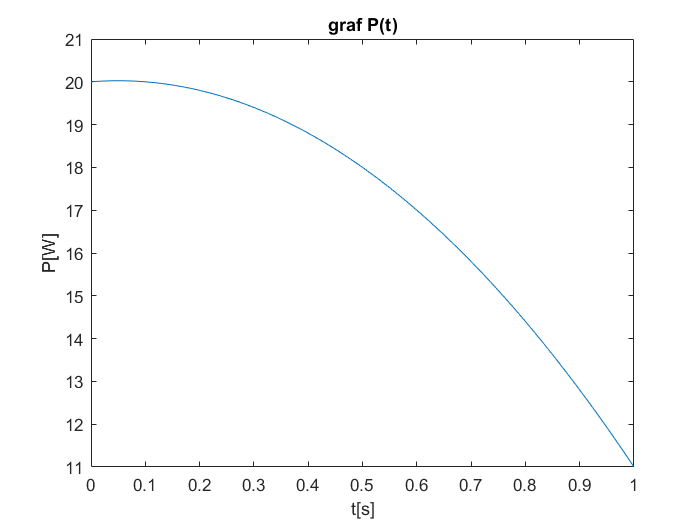
\includegraphics[width=0.8\linewidth]{graff.png}
            
            \label{fig:enter-label}
    \end{figure}
\end{frame}

% 5. Prosojnica: Trapezna formula za integral
\section{Trapezna metoda}
\begin{frame}[fragile]
\frametitle{Trapezna metoda za izračun integrala}
    Formula trapezne metode za izračun integrala:
    \[
    \int_a^b f(x)dx = \frac{\Delta x}{2} \left(f(x_0) + 2f(x_1) + 2f(x_2) + \cdots + 2f(x_{n-1}) + f(x_n)\right)
    \]
    Koda:
    \begin{lstlisting}[language=Matlab]
    sum = 0;
    for index = 1:size(P, 1)
    if index == 1 || index == size(P, 1)
        sum = sum + P(index);
    else
        sum = sum + 2*P(index);
    end
    end
    step = t(2) - t(1);
    integRes = (step/2)*sum
    
    \end{lstlisting}

    Rezultat integrala: $17.1665$
\end{frame}

\end{document}
